% !TEX root = ../partial-sdm.tex

\section{Results (iv): Supervised classification application}

The supervised classification problem consists of categorize data into groups after seeing some samples from each group. First, it is presented pieces of data with their categories. The algorithm learns from these data, which is known as learning phase. Then, new pieces of data are presented and the algorithm must classify them into the already known groups. It is named supervised because  the algorithm will not create the groups itself. It will learn the groups from during the learning phase, in which the groups have already been defined and the pieces of data have already been classified into them.

Although this problem has already been studied (REF), our intention here is to show that a pure SDM may also be used to classify data. \citet{fan1997genetic} has used SDM to solve a classification problem, recognizing handwriting letters from images, but he used a mix of genetic algorithm with SDM, which is very different from the original SDM described by \cite{Kanerva1988}. Even though his algorithm has classified properly, we were intrigued whether a pure SDM would also classify successfully.

Hence, we have developed a supervised classification algorithm based on a pure SDM as our main memory. Our goal was to classify noisy images into their respective letters (case sensitive) and numbers. For some examples, see Figure \ref{fig-classification-examples}.

\begin{figure}[h]
\centering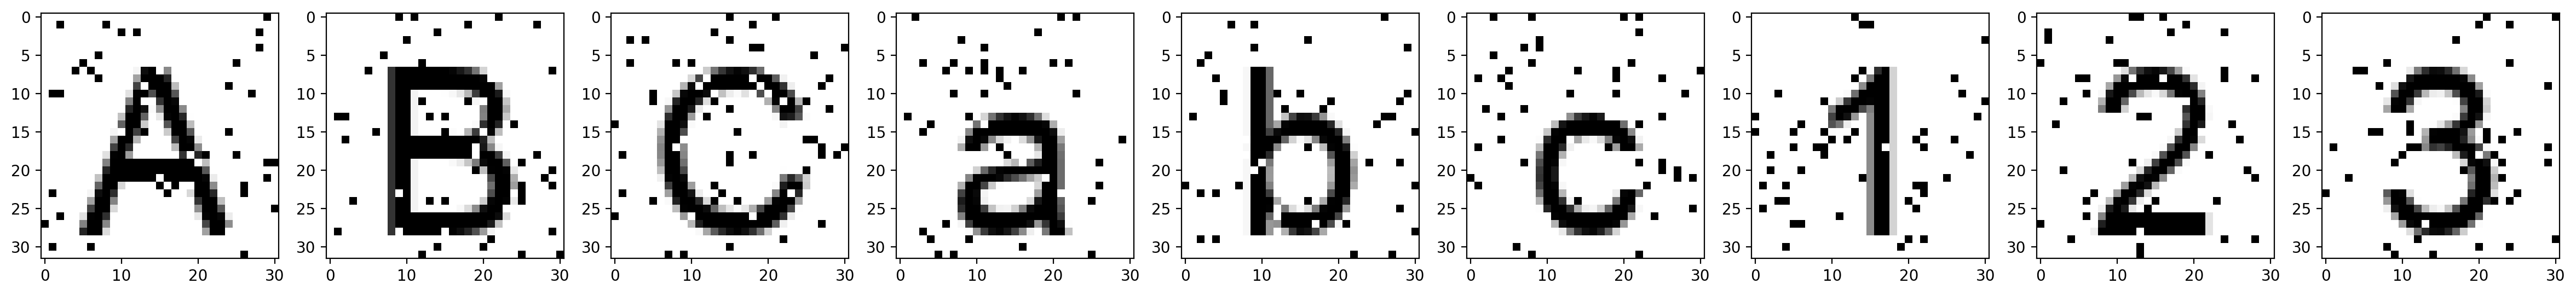
\includegraphics[width=\textwidth]{./images02/classification/example.png}
\caption{Examples of noisy images with uppercase letters, lowercase letters and numbers.
\label{fig-classification-examples}}
\end{figure}

Each image was mapped into a bitstring in which the bits were set according to the color of each pixel of the image. So, white pixels were equal to bit 0, and black pixels to bit 1. This was a bijective mapping (or one-to-one mapping), i.e., there was only one bitstring for each image, and there was only one image for each bitstring.

We had a total of 62 classification group. For each of them, it was generated a random bitstring. Thus, the groups' bitstrings were orthogonal between any two of them.

During the learning phase, we have generated 100 noisy images for each character. For an example, see the generated images for letter A in Figure \ref{fig-classification-training-A}. Then, we have wrote the classification group bitstring into the bitstring associated to each noisy image, i.e., write(bs\_image, bs\_label).

\begin{figure}[h]
\centering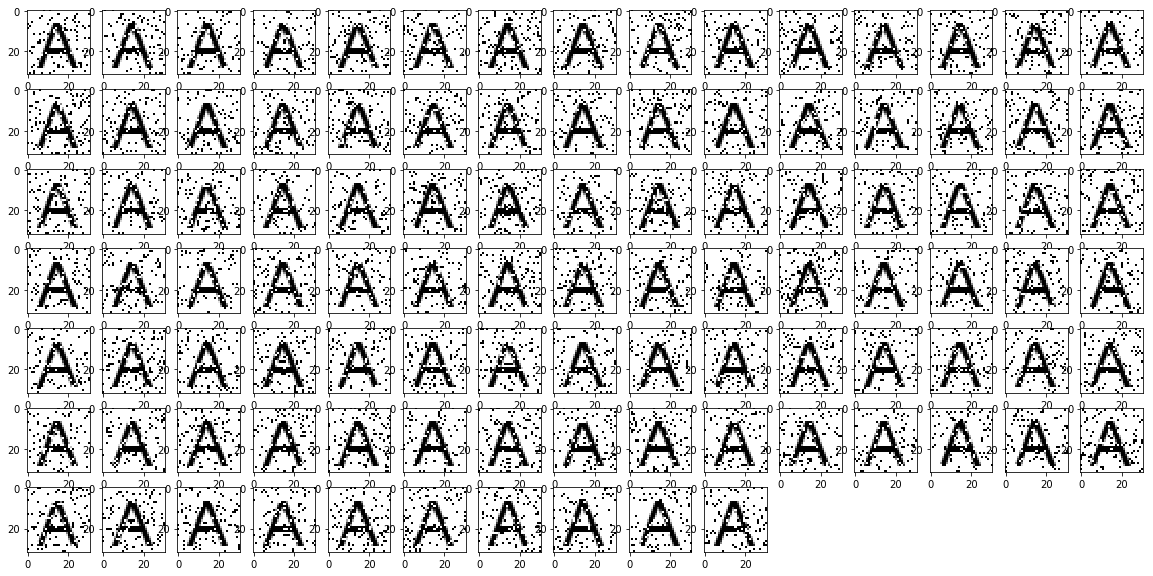
\includegraphics[width=\textwidth]{./images02/classification/trainingA.png}
\caption{100 noisy images generated to train label A.
\label{fig-classification-training-A}}
\end{figure}


\section{Results (iii): Noise filtering application}

\section{Results (v): The possibility of unsupervised reinforcement learning}

